\section{Documento di design}
    \subsection{Architettura del sistema}

    \subsection{Introduzione}
    \begin{flushleft}
        Alla luce delle valutazioni effettuate durante l'analisi dei requisiti, abbiamo trovato conveniente strutturare la nostra app seguendo un tipo di 
        architettura client-server. I client, nel nostro caso, sono quasi sempre dei dispositivi portatili dotati di sistema operativo android (con la possibilità volendo di utilizzare emulatori da pc desktop)
        mentre il server è stato realizzato con il framework di sviluppo Spring Boot.

    \end{flushleft}

    \subsubsection{Client}
    \begin{flushleft}
        Come già detto, il client è composto da un'applicazione android distribuita o tramite apk o tramite play store (rispetta tutti i requisiti per essere pubblicata) che mira ad offrire un'interfaccia utente semplice e pulita 
        per l'accesso agli endpoint forniti dal nostro server Spring-Boot. \\
        In generale, l'architettura di un progetto Android di default segue il pattern architetturale \emph{Model-View-Controller (MVC)}, 
        ma con alcune modifiche per adattarsi al contesto specifico di Android. Talvolta entrano in gioco, come nel nostro caso, altri patter architetturali:\\
        \vspace{1cm}
        \textbf{\emph{Pattern Singleton:}} Abbiamo usato il pattern Singleton per generare una sola istanza del dipendente che si logga nell'app. 
        Cosi facendo, è risultato più semplice aggiornare gli oggetti entità quali Cameriere, Addetto Cucina, Admin e Supervisore e mantenere costantemente un rapporto 1:1 con quanto salvato nel server.\vspace{1cm}
        
        \textbf{\emph{Pattern Observer:}} Molte componenti del sistema Android utilizzano il pattern Observer. 
        Il pattern Observer prevede che un oggetto, chiamato soggetto (Subject), mantenga una lista di oggetti dipendenti, chiamati osservatori (Observers), 
        e che questi vengano notificati automaticamente ogni volta che lo stato del soggetto cambia. In questo modo, 
        gli osservatori possono essere aggiornati in modo efficiente sullo stato del soggetto senza dover verificare continuamente se qualcosa è cambiato.
        In Android, il pattern Observer viene utilizzato, ad esempio, per gestire gli eventi generati dall'utente (come i tap sullo schermo), per notificare i cambiamenti nei dati  o per gestire la comunicazione tra componenti diversi dell'applicazione.
        Anche l'implementazione di \textbf{CallBack} come nel nostro caso (con VolleyCallback) possono essere viste come un' implementazione del pattern Observer.
        Più in particolare la nostra VolleyCallback, che altro non è che un'interfaccia, richiede di implementare in ogni Activity il metodo onResponse() che aggiorna i dati locali con i dati ricevuti dal server.
        Ciò che andiamo ad aggiornare in locale sono poi i Singleton del lavoratore loggato. Da lì, si passa poi all'aggiornamento delle viste nel caso di novità nell'oggetto risposta ricevuto. \vspace{1cm}
       
        \textbf{Volley} Volley è una libreria Android sviluppata da Google che semplifica l'elaborazione di richieste di rete in applicazioni Android. È stata progettata per gestire facilmente le chiamate REST API e può essere utilizzata per inviare e ricevere dati in diversi formati, come JSON, XML e immagini.
        Volley utilizza una combinazione di caching e pooling di connessioni per garantire prestazioni elevate e ridurre il consumo di risorse. Inoltre, supporta la gestione automatica di thread e gestisce in modo trasparente gli errori di rete, semplificando notevolmente la scrittura di codice robusto e affidabile.
        Implementata come Singleton, garantisce l'esistenza di una sola istanza di essa, e ci assicura consumi di memoria costanti e limitati.
        
        \textbf{Gson} Gson è una libreria Java sviluppata da Google che permette la serializzazione e la deserializzazione di oggetti JSON (JavaScript Object Notation) in oggetti Java. Gson offre una serie di metodi per la conversione di oggetti Java in JSON e viceversa, semplificando il processo di scambio di dati tra applicazioni Java e servizi web che utilizzano il formato JSON. 
    \end{flushleft}
    \vspace{0.2cm}


    \subsubsection{Server}
    \begin{flushleft}
        Il back-end della nostra applicazione è stato realizzato con la tecnlogia offerta da Spring Boot, un potente framework di svillupo che sfrutta Java.
        L'architettura che prevede è anch'essa a 3 livelli e prevede i seguenti componenti:
        \begin{itemize}
            \item Model: L'insieme di classi che rappresentano le entità della nostra applicazione. Le stesse sono riportate sul client, e, cosa più importate, spring mappa le classe con annotation "@entity" 1:1 con le tabelle nel db relazionale.\\
                
            \item Repository: Sfruttando il framework JPA (Java Persistence API) riusciamo a gestire persistenza e consistenza dei dati nel db in maniera quasi automatizzata. Spring ci fornisce un gran supporto in questo ambito.
            \item Controller: Qui ci va tutta la logica di controllo del server. Sono queste le classi che espongono gli end-point Rest ai client e, comunicando con le repository aggiornano i model e le tabelle nel db allo stesso tempo.
        \end{itemize}
    \end{flushleft}

    \begin{figure}[H]
        \centering
        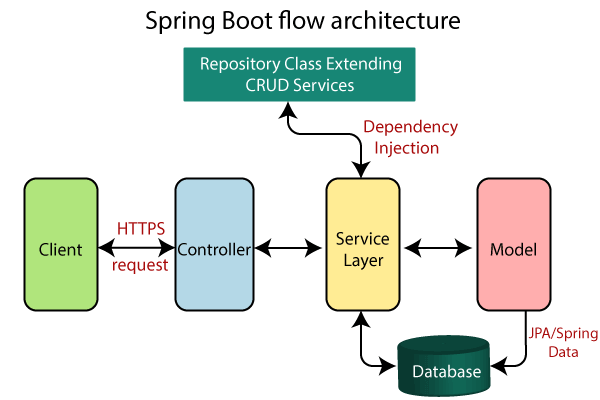
\includegraphics[scale=0.3]{assets/immagini varie/spring-boot-architecture2.png}
        \caption*{\textbf{Figura}: Spring-Boot}\label{fig:spring_Arch}
    \end{figure}

    \begin{flushleft}
        La scelta di utilizzare spring è dovuta principalmente alle sue caratteristiche di flessibilità e scalabilità. Semplifica inoltre lo sviluppo dell'intero applicativo
        grazie alle sue funzionalità di auto-configurazione e di gestione delle dipendenze, che avviene con Gradle e Maven. Spring Boot fornisce inoltre un'ampia gamma di funzionalità per sviluppare applicazioni web in modo rapido e facile. Queste funzionalità includono la gestione delle richieste HTTP, la gestione delle sessioni, la sicurezza e la gestione delle transazioni, tra le altre.
    \end{flushleft}
    

    \newpage

    \begin{flushleft}
        \textbf{Microsoft Azure}\\
        Microsoft Azure è la piattaforma cloud pubblica di Microsoft, che offre servizi di cloud computing. Tra i vari piani che mette a disposizione abbiamo usufruito
        di quello "gratuito" che ci ha permesso di eseguire una macchian virtuale linux (seppur con poche risorse) e un database relazionale, che nel nostro caso è stato PostgreSQL.
        La configurazione della macchina virtuale non ha richiesto particolari abilità: tramite connessione ssh abbiamo configurato il progetto Spring Boot e avviandolo 
        mettiamo a disposizione gli end-point raggiungibili poi dai client.
        La potenza computazionale in questa fase di sviluppo e di utilizzo limitato dell'applicativo potrebbe risultare esile, ma il vantaggio di piattaforme quali
        Azure è possibile in qualsiasi momento aumentare le risorse dedicate a db e/o macchina virtuale, aumentando di fatto la scalabilità della nostra applicazione.
        
    \end{flushleft}

    \begin{figure}[H]
        \centering
        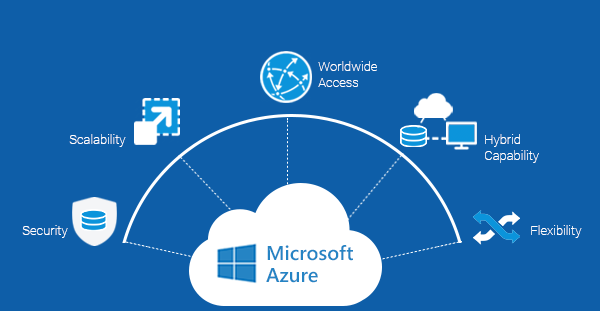
\includegraphics[scale=0.5]{assets/immagini varie/azure loc.png}
        \caption*{\textbf{Figura}: Micrsoft Azure}\label{fig:mic_az}
    \end{figure}
    \newpage
    \begin{flushleft}
        \textbf{E la sicurezza?}\\
        La sicurezza è garantita sia dalla sicurezza intrinseca dei servizi offerti da Microsoft Azure (parliamo quindi di operatività, assistenza, scalabilità) sia da un piccolo sistema di sicurezza pensato dal team:
    \end{flushleft}

    \begin{lstlisting}[language = Java, frame = trBL, firstnumber = last, escapeinside={(*@}{@*)}]
        @Component
        public class AppCodeInterceptor implements HandlerInterceptor {

            private static final String HEADER_APP_CODE = "app_code";
            private static final String EXPECTED_APP_CODE = "Ratatuille23";

            @Override
            public boolean preHandle(HttpServletRequest request, 
            HttpServletResponse response, Object handler) throws Exception {
                String appCode = request.getHeader(HEADER_APP_CODE);
                if (appCode == null || !appCode.equals(EXPECTED_APP_CODE)) {
                    System.out.println("Access denied");
                    response.setStatus(HttpStatus.UNAUTHORIZED.value());
                    return false;
                }
                return true;
            }
            
            // Override degli altri metodi dell'interceptor se necessario
        }
    \end{lstlisting}
    

    \begin{flushleft}
        Questa piccola parte di codice presente nel back-end, ci garantisce che nessun'altra richiesta al di fuori da 
        quelle effettuate con il parametro "appcode" da noi definito sul client venga accettata.
        Estranei e malintenzionati, riceveranno lo status 401 se proveranno ad accedere a qualunque dei nostri endpoint.
    
    \end{flushleft}

   
        
    